\section{Evaluation}\label{sec:eval}
\subsection{Survey}\label{sec:survey}
To evaluate the performance of the agent, a sample dataset of potential user inputs and agent outputs 
was produced.  A description of each input can be found in \autoref{tab:evaltests}. Random sampling 
was used to produce baseline recommendations.  These were 
used in a survey which 30 whisky enthusiasts completed.\footnote{See \autoref{sec:StatementOnEthics}
regarding ethics.}.
They were asked to rate each recommendation on the basis of the corresponding input.  
While the agent recommends 10 whiskies by default, only 3 recommendations were given from the baseline and agent
to avoid making the survey too cumbersome.

\begin{table}
    \centering
    \caption{Description of inputs in evaluation dataset.}\label{tab:evaltests}
    \begin{tabular}{p{0.1\linewidth} p{0.7\linewidth}} 
    \toprule
    Input Reference & Rationale                                                                                                                                 \\ 
    \hline
    ATN1            & Replicating a user who has tried and developed tastes for a variety of whiskies available at supermarkets, but hasn't tried much beyond.  \\
    ATN2            & Replicating a significant partiality towards heavily peated whiskies.                                                                     \\
    ATN3            & Replicating an enjoyment of both peated and sherried whiskies.                                                                            \\
    ATN4            & A user with niche and specific whisky tastes.                                                                                             \\
    GC              & Producing recommendations based on general inputs without considering specific tasting notes.                                            \\
    DD1             & Dream Dram recommendation from a very peat heavy input.                                                                                   \\
    DD2             & Dream Dram recommendation describing a very oily and fruity whisky.                                                                       \\
    \bottomrule
    \end{tabular}
\end{table}

Participants were given all information available to the 
agent for each output including description and tasting notes (and some information the agent does not use such as 
ABV, Price etc), however they were instructed not to factor price in their ratings as price parameters were set 
by the hypothetical user. There was an option to leave text feedback.

\subsection{Results}\label{sec:res}

As can be seen in figures \ref{fig:allrec} and \ref{fig:avgrec}, most recommendations were rated higher than 
the mean baseline. 

A paired one-tailed t-test was conducted on the baseline scores and corresponding recommender scores for
each sample input. There was a significant increase in scores from the recommender ($M=6.28$, $SD=1.13$)
compared with the baseline ($M=4.71$, $SD=1.15$), $t(12) = 2.22$, $p<0.05$. There was a mean increase of $1.57$ 
points.

\begin{figure}[!htb]
    \centering
    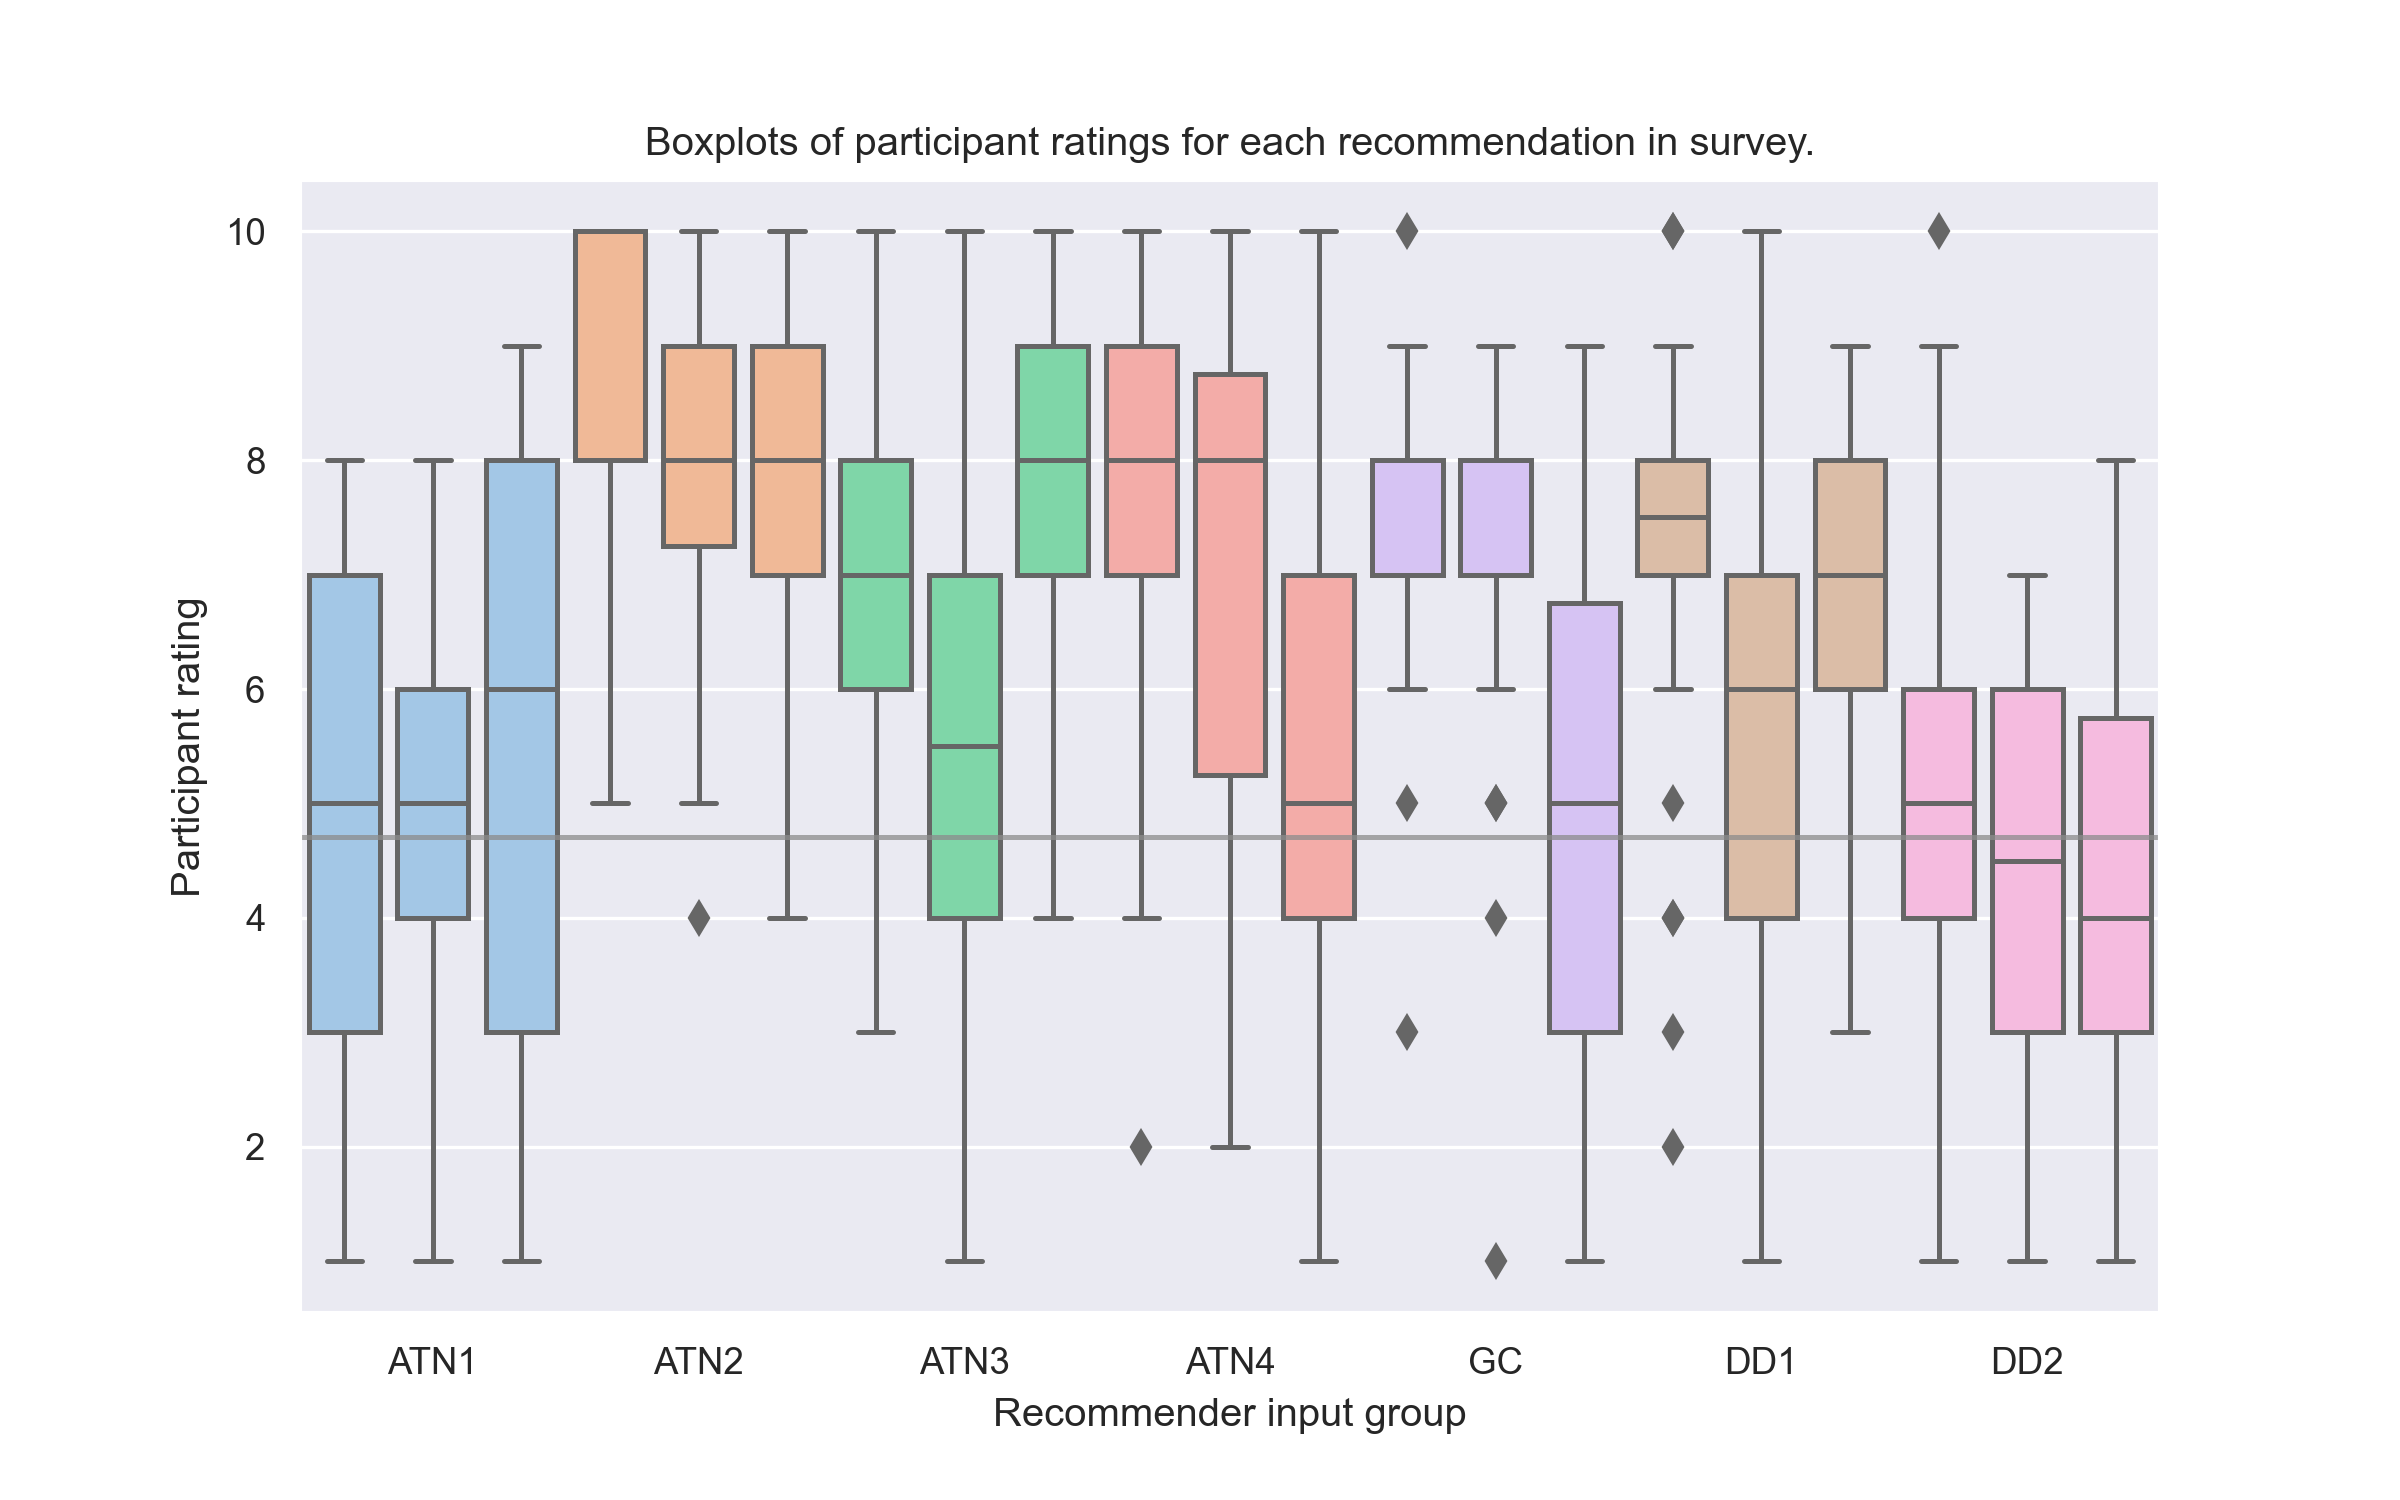
\includegraphics[width=0.8\textwidth]{graphics/all_recommendations}
    \caption{Boxplots of participant ratings for each recommendation, grouped by sample input. The grey line 
    indicates the mean baseline rating.}\label{fig:allrec}
\end{figure}

\begin{figure}[!htb]
    \centering
    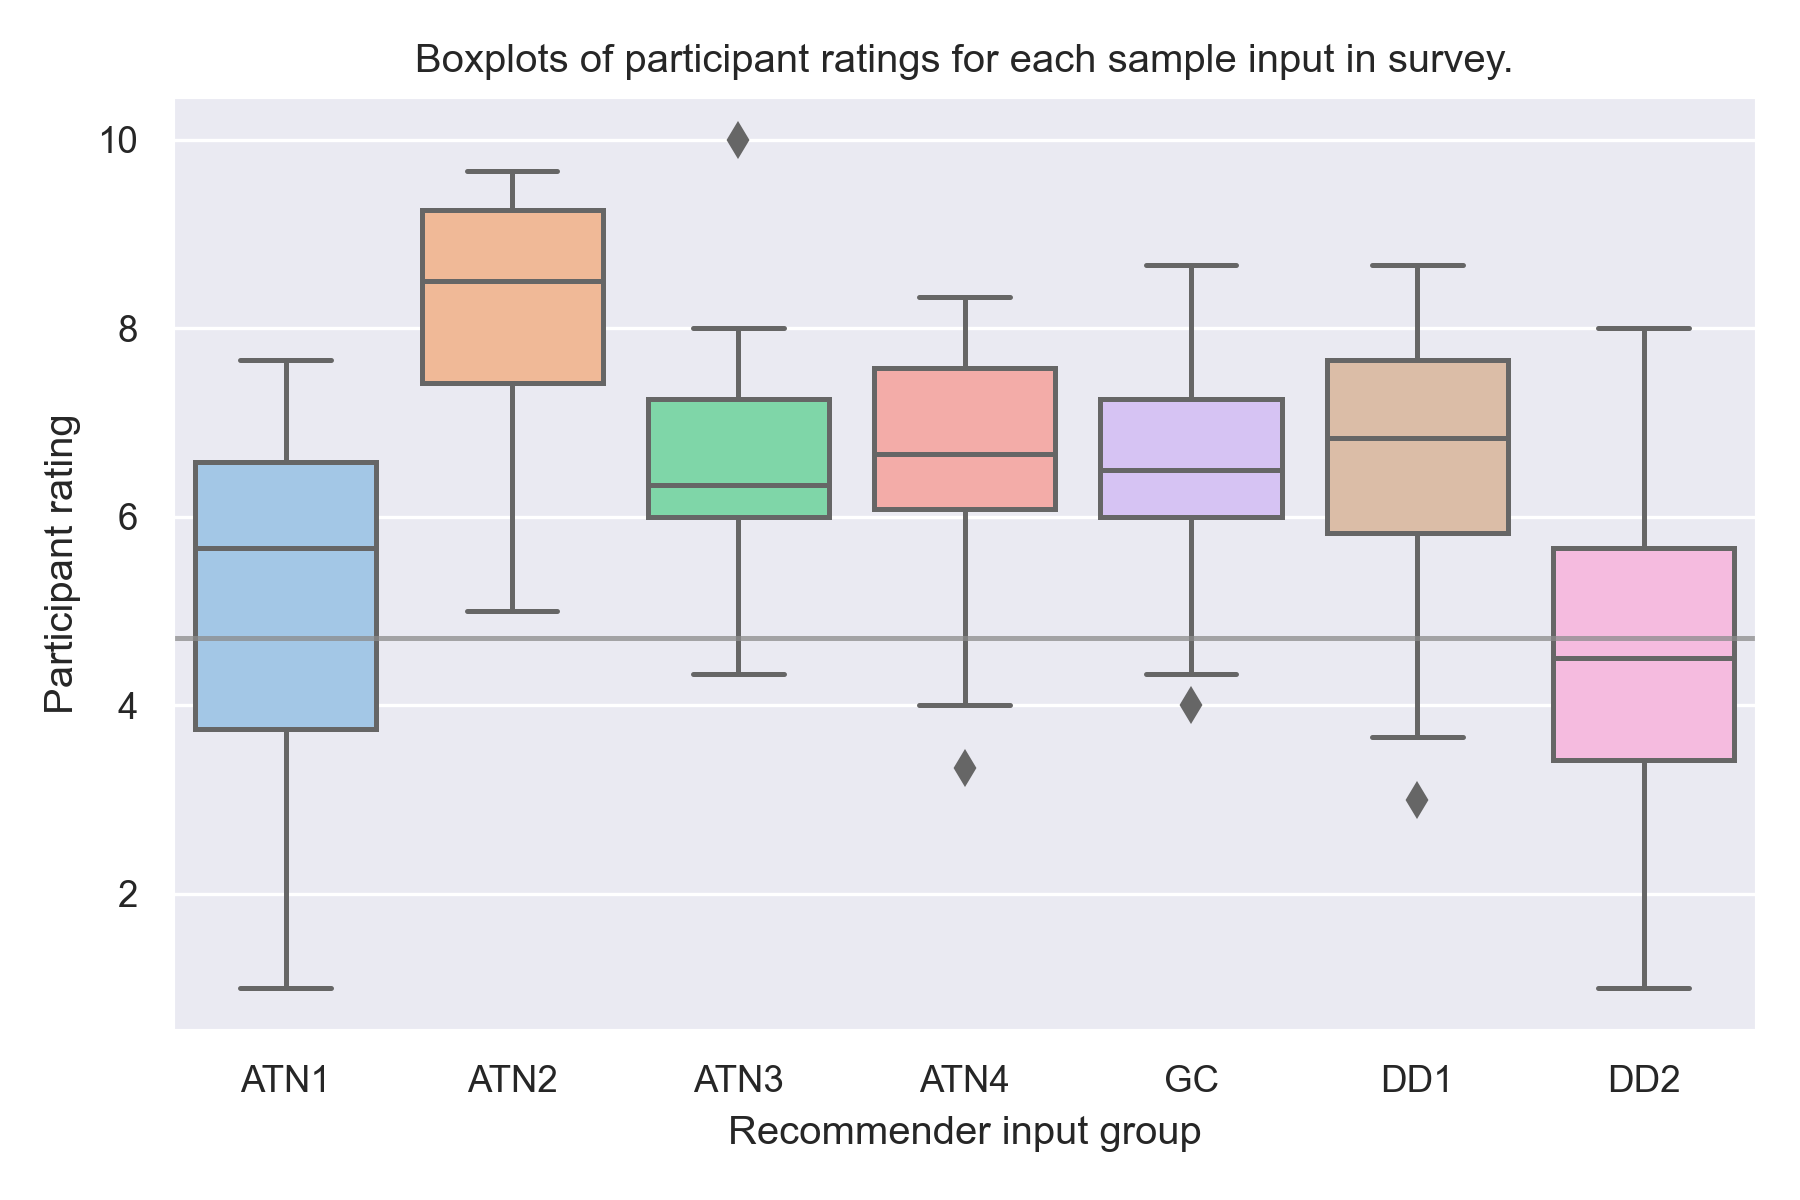
\includegraphics[width=0.8\textwidth]{graphics/avg_recommendations}
    \caption{Boxplots of participant ratings for each sample input. The grey line 
    indicates the mean baseline rating.}\label{fig:avgrec}
\end{figure}

\subsection{Discussion}\label{sec:disc}
Despite promising results, it is clear that some 
recommendations received a large range of ratings.  The small samples used, both of enthusiasts and 
inputs/recommendations, are far from ideal.

On reading the free-text responses, it's clear that some participants weren't confident
in their whisky knowledge. Similarly some participants hadn't followed the instructions, for example
one participant stated they had penalised recommendations with high prices.

A few interesting points were made which are worth considering.  One participant suggested that the input
for ATN1 was contradictory, perhaps explaining its relatively low score. This suggests that (as intended) this 
recommender method is not ideal for taking a users entire taste profile, 
rather recommending a whisky to try based on similarity between a small number of tried whiskies.  It would
be interesting to investigate whether such a system is possible in the specific case of whisky.

Many users pointed out that many recommendations were very niche, suggesting an extra filter could be
incorporated allowing a user to filter out single-cask/independent bottles.  This also could have impacted
the accuracy of participant's scores.